\section{The Chosen Tests}
The tests are a mixture of general functionality and two specific algorithms. This section assumes that the reader is familiar with the Big O notation.

\subsection{Language Overhead}
Each programming language has an overhead startup cost. This is measured by submitting code which does the minimum given this context. In Figure \ref{fig:language_overhead} a minimum code block for the C\# programming language is demonstrated.

\begin{figure}[h]
	\lstset{style=sharpc}
	\begin{lstlisting}
	public class OverheadTest{
		public string SimpleReturn(string input){
			return "";
		}
		public static void Main(){}
	}
	\end{lstlisting}
	\caption{C\# code for language overhead testing.}
	\label{fig:language_overhead}
\end{figure}

This code will recieve an empty string as input, and return an empty string. Measuring the overhead makes it possible to compensate for a language which has a slower execution time. For example, it would be unfair to restrict Python code to the same time-limit as C\# code, since Python has a considerably longer startup time than the native .NET language C\#. 

\subsection{Common Operators}
The common operators are addition (+), subtraction (-), multiplication (*), division (/) and modulo (\%). This test will measure how the language performs doing the simplest operations, giving an indication of its general performance. Figure \ref{fig:addition_test} shows the code used for the addition test in Python.

\begin{figure}[h]
	\lstset{style=sharpc}
	\begin{lstlisting}[language=python]
	class AdditionTest:
	    def AddNumbers(self, input):
	        input = input.split(" ")
	        array = list(map(int, input))
	        total = sum(array)
	        return str(total)
	\end{lstlisting}
	\caption{Python code for testing the addition operation.}
	\label{fig:addition_test}
\end{figure}

This code takes a string containing numbers as input, divides it into an array of numbers, sums these numbers and returns this sum.

\subsection{Insertion Sort}
Insertion Sort is a comparison based sorting algorithm useful for sorting small inputs. The algorithm can be expressed using code, but this doesn't illustrate it very well for people not already familiar with it, so instead I will explain it using playing cards (using a common 52 card deck):

\begin{itemize}
\item Start with an empty left hand and imagine yourself seeing a bunch of cards on a table.
\item Pick a card from the table one at a time from left to right.
\item Insert this card into the correct position in your left hand.
\item The correct position is determined by comparing this card to each other card in your hand from right to left.
\item The cards in your left hand are always sorted before each new card is picked.
\end{itemize} 

The algorithm has a runtime of $O(n^2)$ but can still outperform more advanced algorithms such as Merge Sort (described in section \ref{subsec:merge_sort}) because Merge sort has an extra overhead from its recursive function calls and also uses more memory, but this is only true for small inputs (what ``small'' is varies from system to system) \cite{Insertionsort}.

Insertion Sort is a suitable algorithm for testing performance between different languages since its implementation is very simple, straightforward and similar in these languages.


\subsection{Merge Sort} \label{subsec:merge_sort}
Merge Sort is a divide and conquer, comparison based sorting algorithm. It's stable in the sense that it preserves the input order of equal elements in the output. The algorithm goes as follows (once again using the common 52 card deck):

\begin{itemize}
\item Imagine yourself seeing a full deck of cards in a line on a table.
\item Divide the cards into two equally sized piles. There should now be 26 cards on your left side and 26 cards on your right side.
\item Keep dividing these piles in half until you only have piles with one card in them. 
\item Now merge these one card piles together so that you end up with a pile that contains 2 cards that are sorted from left to right (in ascending order).
\item Keep merging all piles together until you end up with one pile containing all of the cards (52) in sorted order.

\end{itemize} 

Figure \ref{fig:mergesort} illustrates this process using eight cards.

\begin{figure}[h]
	\centering
	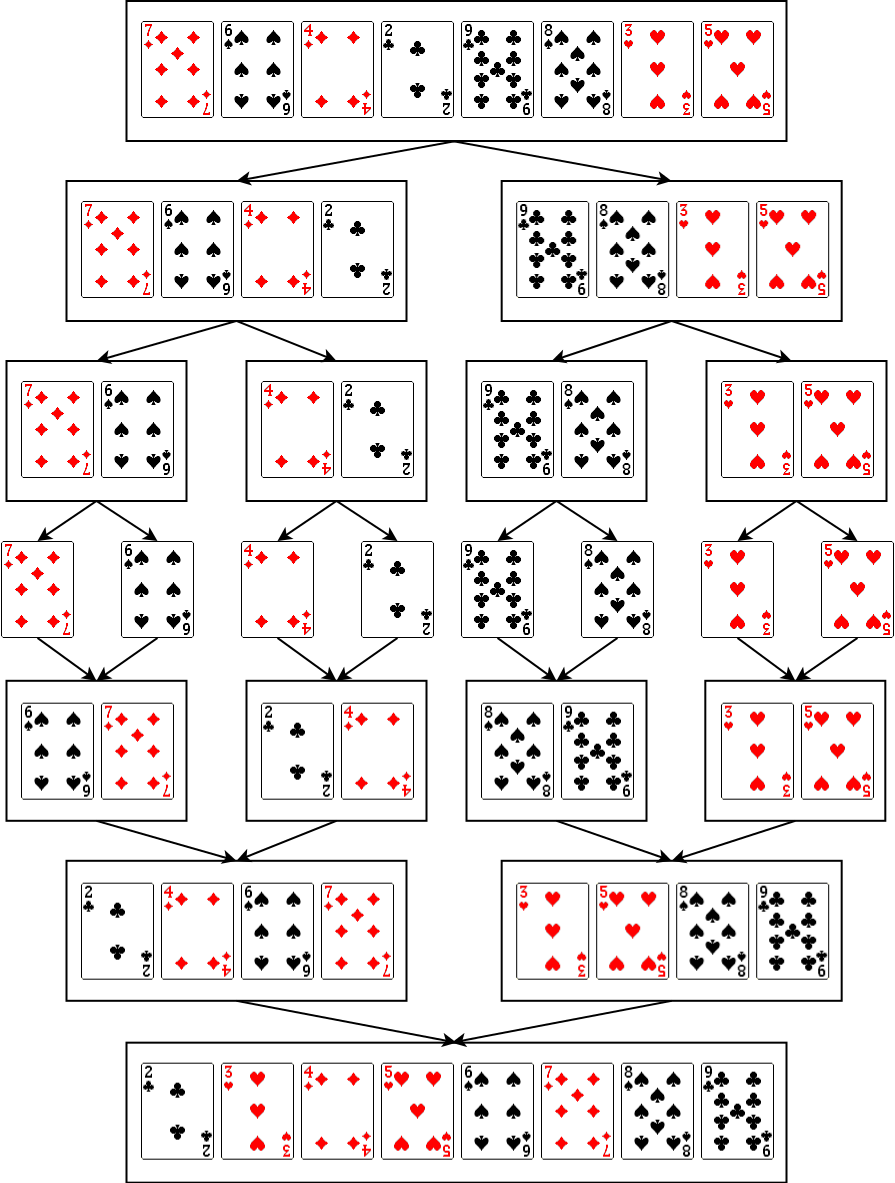
\includegraphics[width=0.9\linewidth]{chapters/media/mergesort4.png}
	\caption{Illustration of the Merge Sort algorithm using eight cards. The cards are subsequently divided up and then merged back together in sorted order.}
	\label{fig:mergesort}
\end{figure}

There are several sorting algorithms that have a worst time complexity of $O(n * log(n))$, Merge Sort was chosen because it has an auxiliary worst space complexity of $O(n)$, thus using more memory than other similar algorithms (e.g. Heap Sort) \cite{Mergesort}. This helps in illustrating how different programming languages differ in memory consumption.





